%#!pdfplatex
\documentclass{article}
\usepackage{graphicx}
\title{Fundamental Exercise on Computer and Information Engineering 1B \\ Image Processing}
\author{XL15613   Thiago Machado da Silva}
\date{\today}

\begin{document}
\maketitle

\section*{Output}
In Figure~\ref{fig:output} the executions reports no error. The randomWalk, photo-edge and photo-edge-thick images were constructed properly. The randomWalk image reminds me of {\tt xscreensaver's "Wander"} animation, where there is only one walker, but it changes the color from time to time, and it appear in the opposite side of the screen when one side is reached. \\
\begin{figure}[htbp]
  \makebox[\textwidth][c]{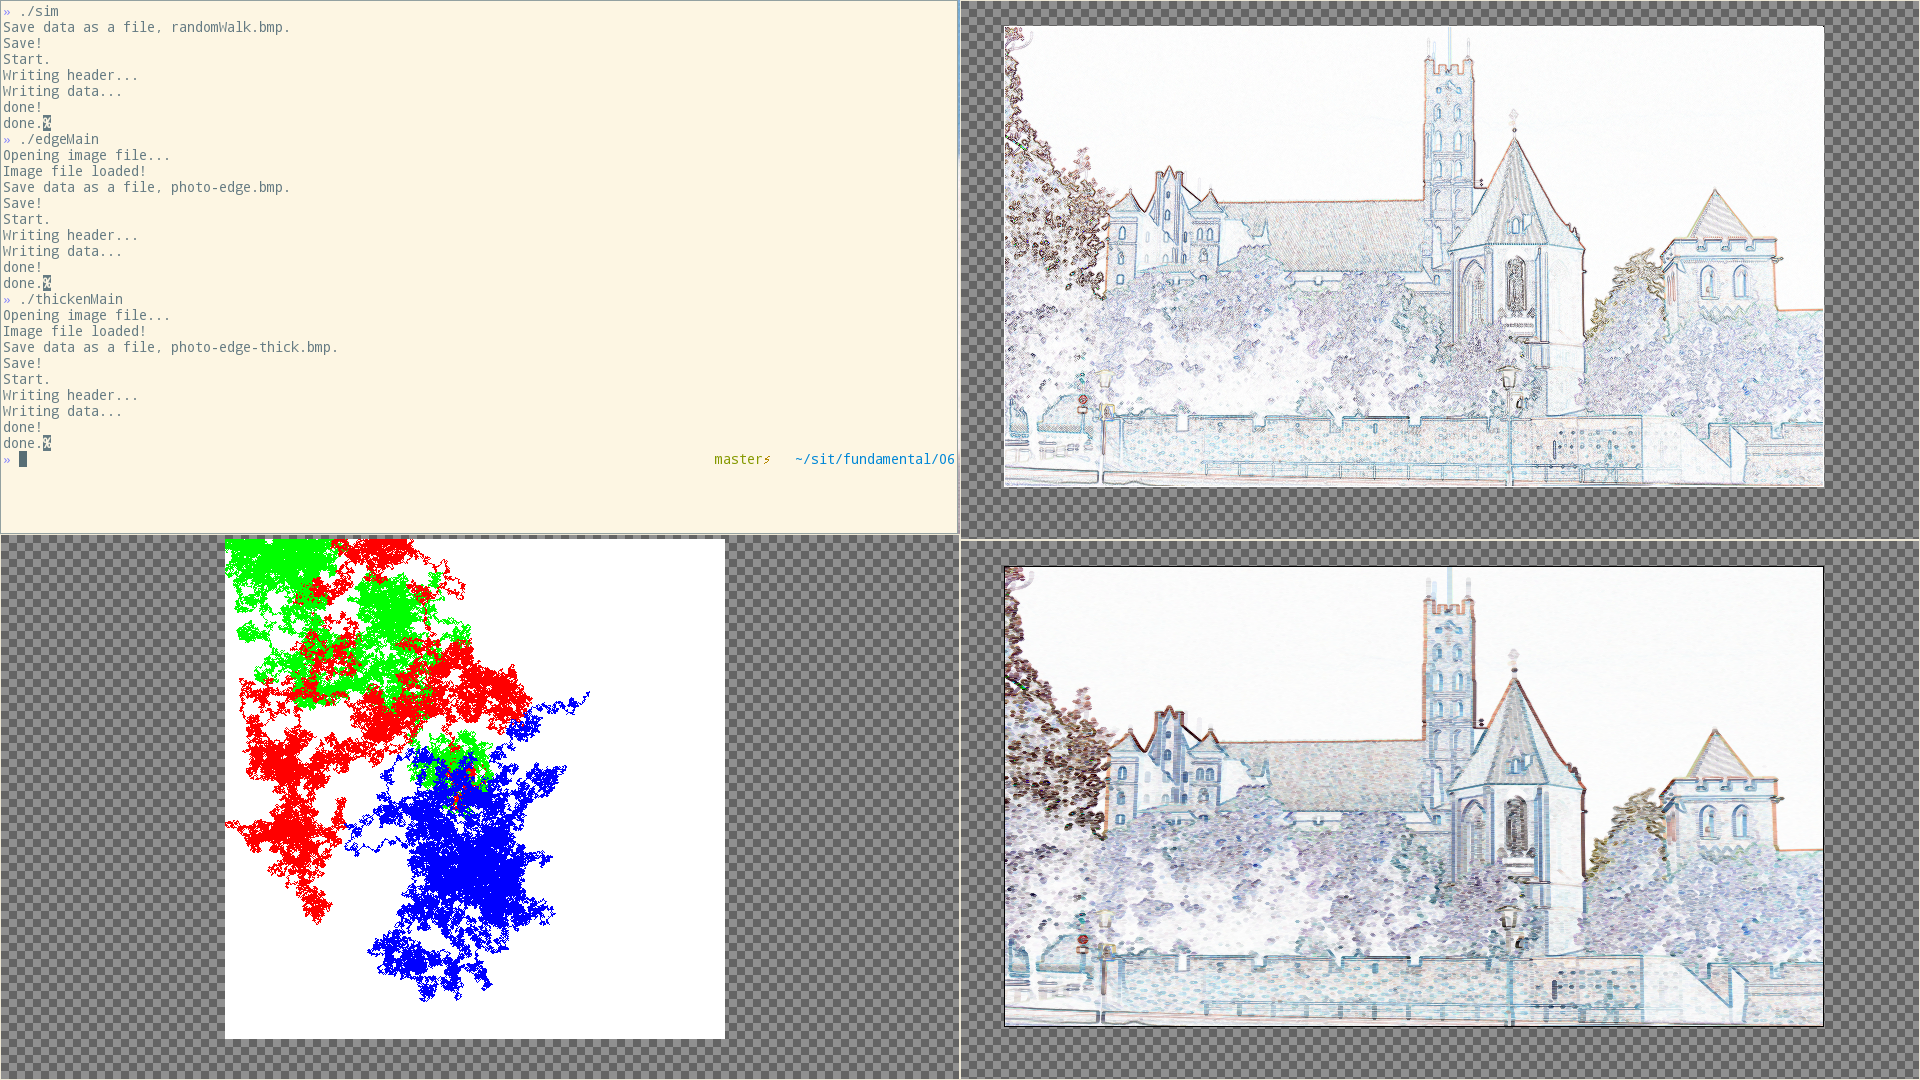
\includegraphics[width=1.78\textwidth]{./output.png}}%
  \centering
  \caption{from top to bottom, left to right: programs' outputs, {\tt randomWalk.bmp}, {\tt photo-edge.bmp} and {\tt photo-edge-thick.bmp}.}
  \label{fig:output}
\end{figure}

\section*{Source codes}
Shown in Figure~\ref{fig:src1} and Figure~\ref{fig:src2}.

\begin{figure}[h]
  \makebox[\textwidth][c]{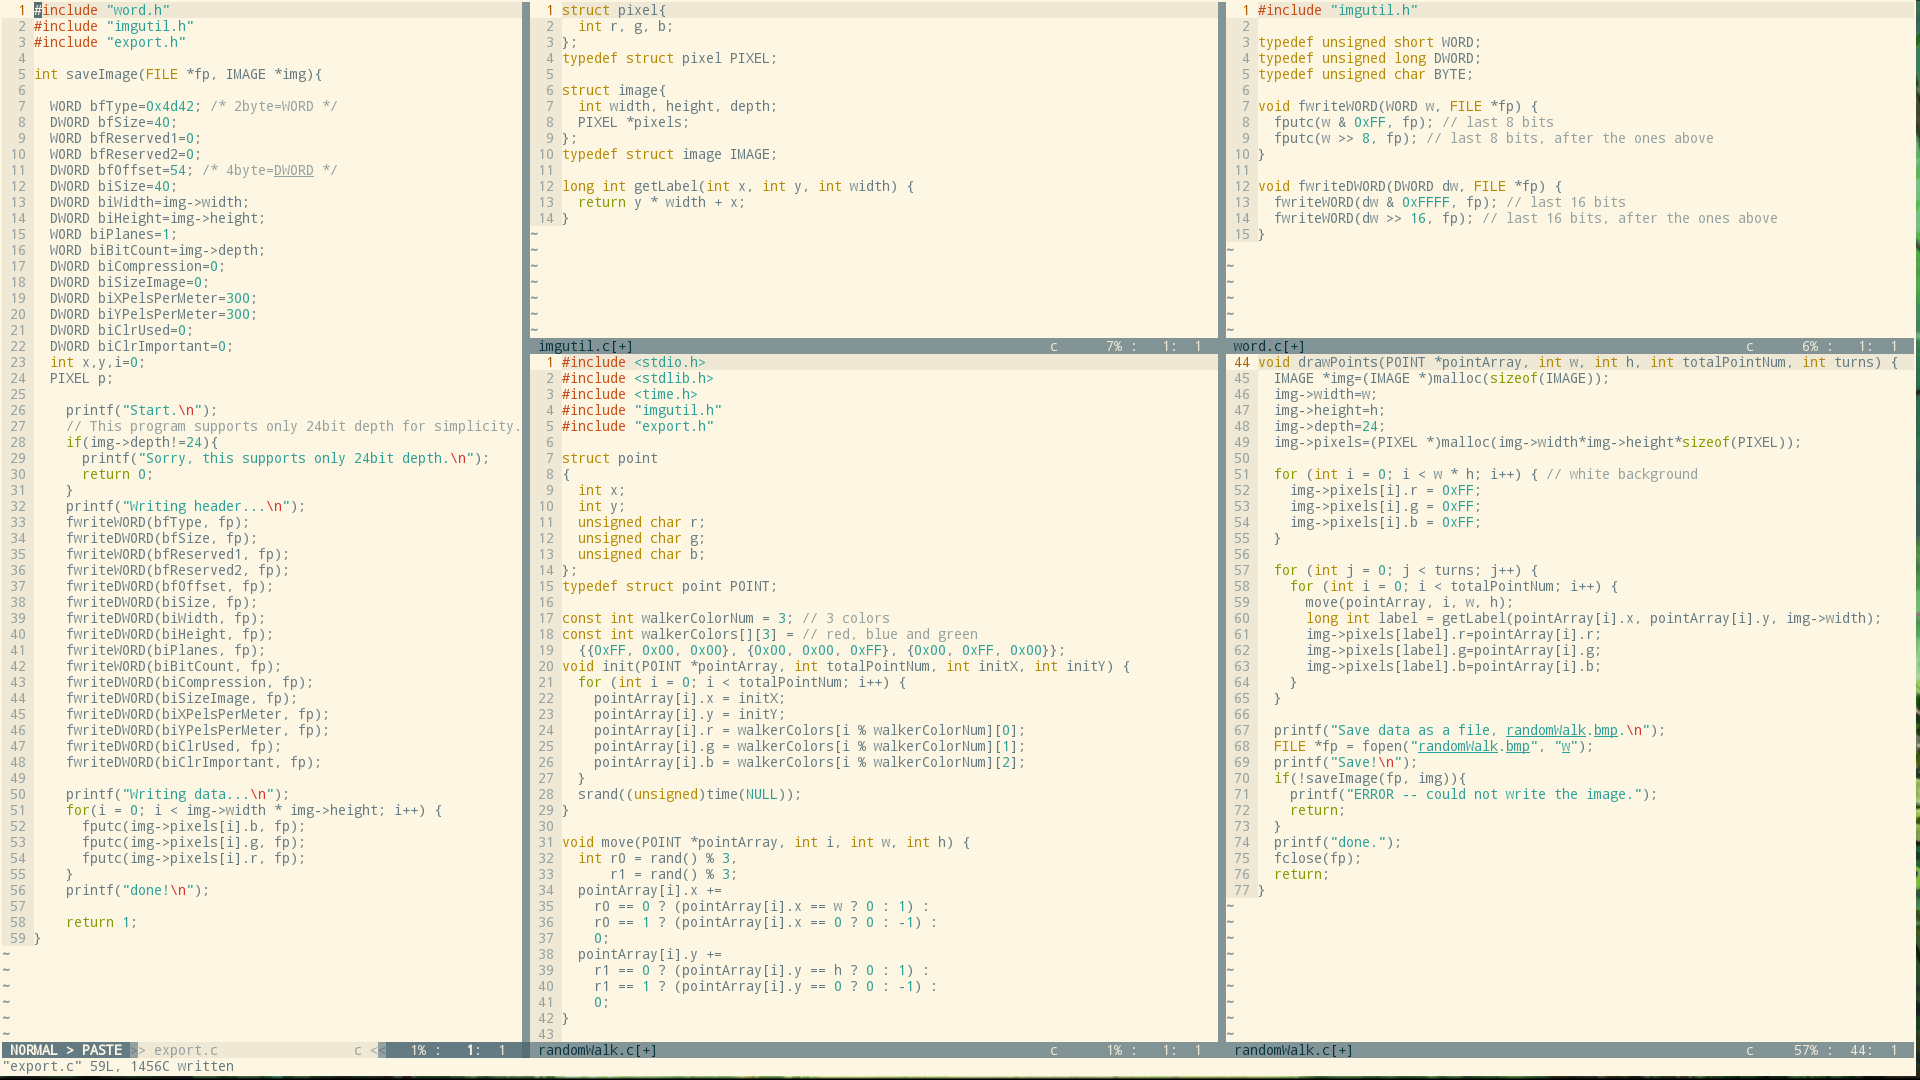
\includegraphics[width=1.78\textwidth]{./src1.png}}%
  \centering
  \caption{from left to right, top to bottom: {\tt export.c}, {\tt imageutil.c}, {\tt word.c}, {\tt randomWalk.c} (until line 43) and {\tt randomWalk.c} (from line 44).}
  \label{fig:src1}
\end{figure}

\begin{figure}[h]
  \makebox[\textwidth][c]{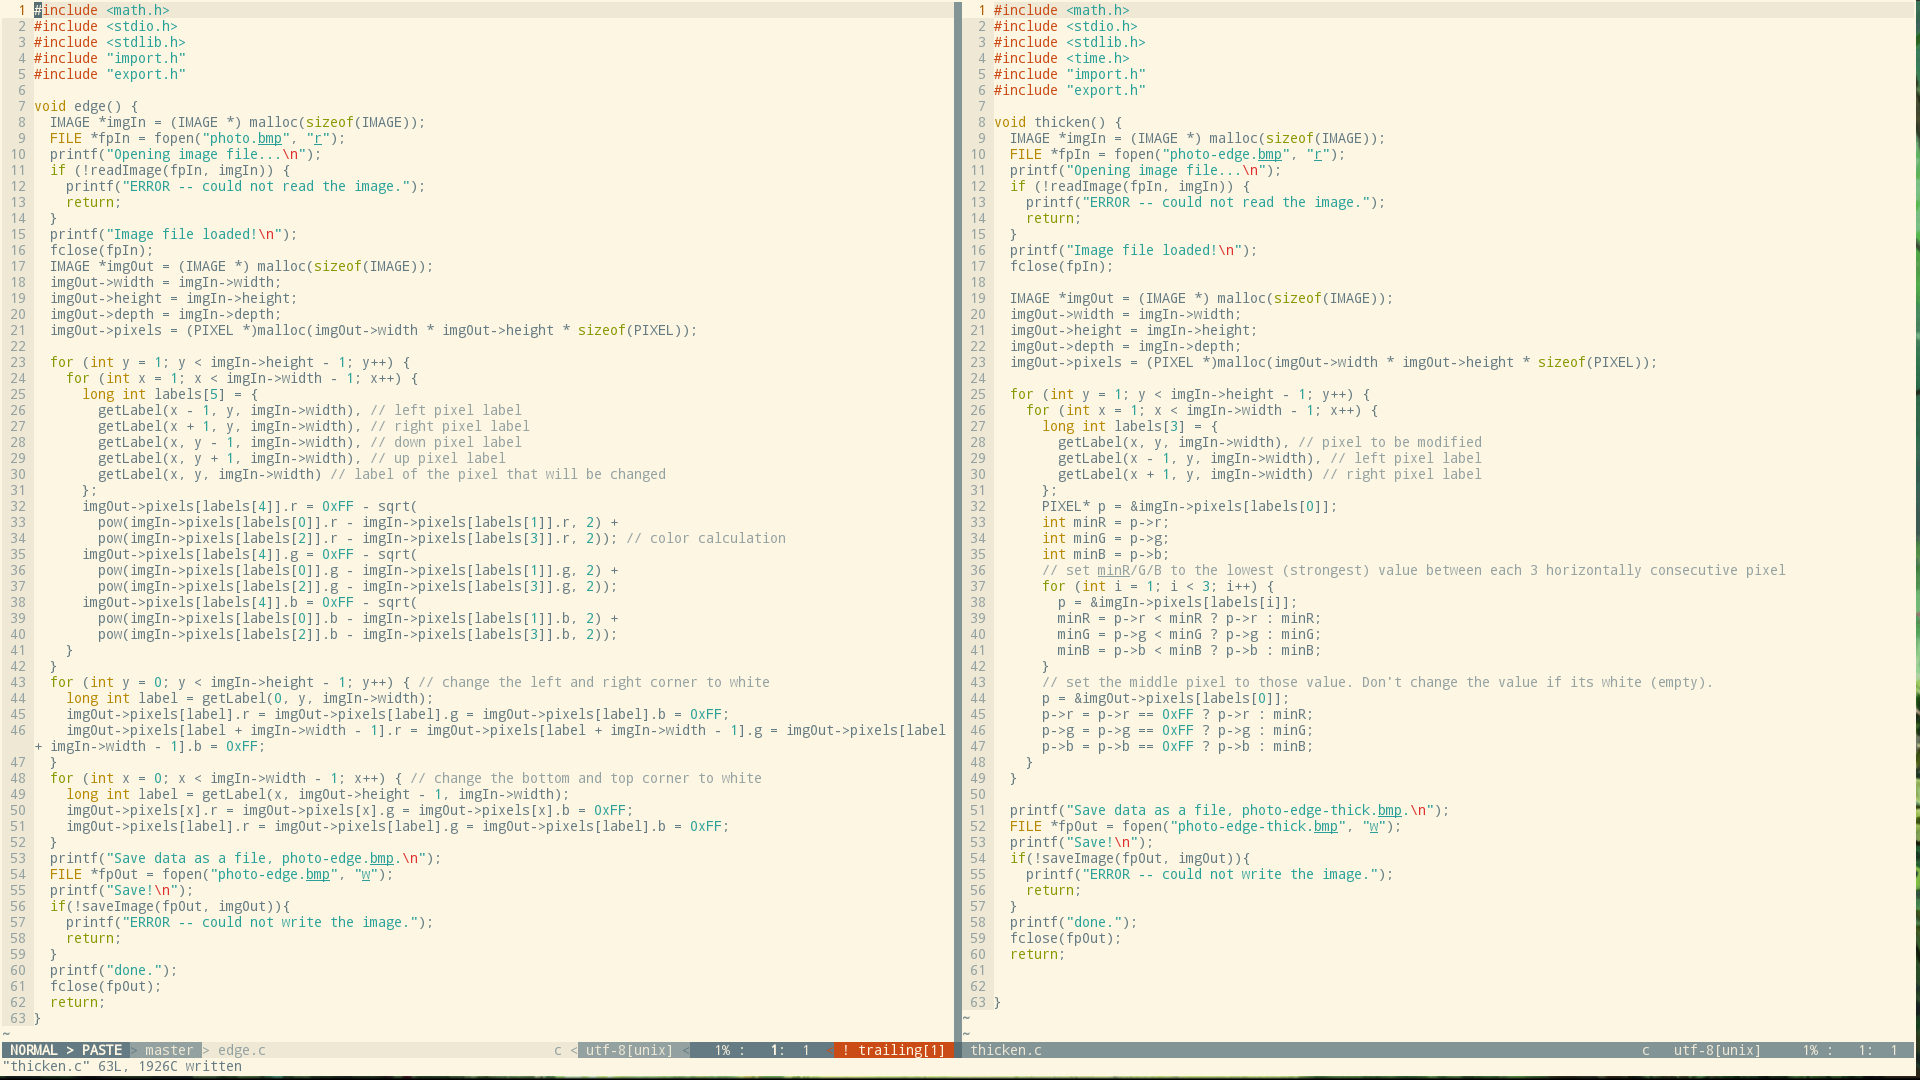
\includegraphics[width=1.78\textwidth]{./src2.png}}%
  \centering
  \caption{from left to right: {\tt edge.c} and {\tt thicken.c}.}
  \label{fig:src2}
\end{figure}

\end{document}
